We now attack the C reference implementation of MEDS,\footnote{\url{https://github.com/MEDSpqc/meds}}
exploiting the tree-traversal logic of the path construction --- \chg{line~\ref{alg:meds:path}} of
Algorithm~\ref{alg:sign_meds} --- to leak hidden seeds. In that
implementation, path generation and tree reconstruction are not two functions
but two modes of one, \texttt{stree\_to\_path\_to\_stree}, selected by a
\texttt{mode} parameter; Listing~\ref{lst:path} gives the traversal.

\begin{lstlisting}[style=cstyle,caption={Traversal loop of \texttt{stree\_to\_path\_to\_stree}; highlights mark the three fault targets.},label=lst:path]
void stree_to_path_to_stree(uint8_t *stree, ..., uint8_t *path, int mode) {
    while (1==1) {
        int index_leaf = 0;
        `\label{lst:path:while}\highlight{yhl}{while ((indices[id] \chg{>{}>} (MEDS\_seed\_tree\_height-h)) == i)}` 
        {// Traverse down toward the secret leaf
            h += 1;
            i <<= 1;
            if (h > MEDS_seed_tree_height) {
                h -= 1;
                i >>= 1;
                `\label{lst:path:inc}\highlight{rhl}{if (id + 1 < MEDS\_w) id++; }`
                `\label{lst:path:leaf}\highlight{bhl}{index\_leaf = 1;}` // Flag node as hidden
                break;
            }
        }
        ...
    }
}
\end{lstlisting}

The algorithm identifies the secret leaves ($h[i] > 0$) and performs a
depth-first search, halting as soon as it reaches a node that is no longer an
ancestor of the current hidden leaf and appending that node to the path. On
reaching a hidden leaf it sets \texttt{index\_leaf}, so the leaf seed stays
unpublished, and moves to the next one.

Our objective is to manipulate the control flow so that unpublished seeds ---
internal nodes or leaves --- are written into the public signature path.

\paragraph{Threat model and what a successful fault yields.}
\revon
Our \emph{intended} attack scenario is a victim device that signs a requested
message and emits the resulting output despite a fault. The experiments
below instead glitch a standalone invocation of the publication routine,
using a fixed tree, salt and challenge; no full signing operation is run.
In the intended attack, the adversary does \emph{not} need the
emitted signature to be valid, a point that matters for
\revoff
Section~\ref{sec:counter}: $\resp_i = (\mu_i,\nu_i)$ is present for every
hidden round regardless of the fault, so once the corrupted path discloses
$\sigma_i$ for one such round the extraction of~\eqref{eq:meds-extract}
succeeds even if the digest check would reject. What the adversary needs is
not a valid signature but an \emph{emitted} one.

\paragraph{Experimental Setup.}
Our experimental platform consists of a CW303-STM32F3 target board carrying an
ARM Cortex-M4 STM32F303RCT7 processor. Clock glitching is
performed using a ChipWhisperer-Lite.

\revon
\paragraph{Experimental scope.}
The board executes only the seed-path routine with fixed tree, salt and
challenge. Locating the vulnerable instruction after a complete signing
operation, producing a serialized faulted signature and recovering secret
components on-device were not tested. Thus the measured routine-level yields
cannot be read as end-to-end attack probabilities. Other hardware fault work
on this family has likewise isolated subfunctions~\cite{BandaBK26}.
\revoff

%\subsection{Fault Models}
\paragraph{Fault Models.}
We propose three fault models targeting different stages of the tree traversal.

\noindent\textbf{Model 1: Full Tree Recovery (Root Leakage).}
This attack aims to reveal the root seed, which effectively compromises the entire tree. By injecting a fault that causes the skip of the first iteration of \highlight{yhl}{\texttt{while} loop} at \chg{line~\ref{lst:path:while}} of Listing~\ref{lst:path}, the DFS halts immediately at the root ($h=0, i=0$). The root is incorrectly identified as a node ready for publication.

\noindent\textit{Detection and recovery.} The signature path contains only a
single non-zero element. The adversary confirms the fault offline by expanding
that seed into a full tree, recomputing the round commitments, and checking
them against the digest $d$ carried in the signature; no interaction with the
device is required. Note that the resulting path does not deserialise
correctly under an honest $\PathToSeedTree_t$, so this fault is detectable by
the signer --- see Section~\ref{sec:counter}.

\noindent\textbf{Model 2: Subtree Recovery.}
By glitching the guarded increment \highlight{rhl}{\texttt{id++}} at \chg{line~\ref{lst:path:inc}}
of Listing~\ref{lst:path}, the algorithm fails to advance the cursor
\texttt{id} into the list of hidden leaves. The traversal logic becomes desynchronized, resulting in the algorithm treating subsequent branches as public. All leaves to the right of the faulted \texttt{id} become computable.

\noindent\textit{Detection and recovery.} This fault is harder to recognise
than the other two, since the path has a plausible length. The adversary can
nonetheless simulate the reconstruction for each of the $w$ possible faulted
values of \texttt{id} and keep the one whose recomputed commitments match $d$,
at a cost of at most $w$ verifications.

\begin{figure}[!tb]
\centering
\begin{tikzpicture}[x=0.6cm, y=0.75cm]
  \tikzstyle{neutnode} = [circle, draw=gray!60, fill=nodehid, text=black, minimum size=12pt, inner sep=0pt, font=\scriptsize]
  \tikzstyle{faulted_leaf} = [circle, draw=red!60, fill=nodehid, text=black, minimum size=12pt, inner sep=0pt, font=\scriptsize]
  \tikzstyle{pubnode}  = [circle, draw=green!50!black, fill=nodepath, minimum size=12pt, inner sep=0pt, font=\scriptsize]
  \tikzstyle{fpubnode}  = [circle, draw=red!50!black, fill=nodepath, minimum size=12pt, inner sep=0pt, font=\scriptsize]
  \tikzstyle{zeronode} = [circle, draw=gray!60, fill=nodepub, minimum size=12pt, inner sep=0pt, font=\scriptsize]
  \tikzstyle{treeedge} = [gray!40, rounded corners=2pt,->, thin]
  \tikzstyle{leaflbl}  = [font=\tiny, below=1pt]
  \node[neutnode](s0) at (3.5,0){$s_0$};
  \node[neutnode](s1) at (1.5,-.75){$s_1$};
  \node[fpubnode](s2) at (5.5,-.75){$s_2$};
  \node[neutnode](s3) at (.5,-1.5){$s_3$};
  \node[fpubnode] (s4) at (2.5,-1.5){$s_4$};
  \node[zeronode](s5) at (4.5,-1.5){$s_5$};
  \node[zeronode] (s6) at (6.5,-1.5){$s_6$};
  \node[pubnode] (s7) at (0,-2.4){$s_7$};
  \node[faulted_leaf](s8) at (1,-2.4){$s_8$};
  \node[fpubnode](s9) at (2,-2.4){$s_9$};
  \node[zeronode](s10) at (3,-2.4){$s_{10}$};
  \node[leaflbl] at (0,-2.9){$\eseed_0$};
  \node[leaflbl] at (1,-2.9){$\eseed_1$};
  \node[leaflbl] at (2,-2.9){$\eseed_2$};
  \node[leaflbl] at (3,-2.9){$\eseed_3$};
  \node[leaflbl] at (4.5,-2.0){$\eseed_4$};
  \node[leaflbl] at (6.5,-2.0){$\eseed_5$};
  \draw[treeedge](s0)--(s1);\draw[treeedge](s0)--(s2);
  \draw[treeedge](s1)--(s3);\draw[treeedge](s1)--(s4);
  \draw[treeedge](s2)--(s5);\draw[treeedge](s2)--(s6);
  \draw[treeedge](s3)--(s7);\draw[treeedge](s3)--(s8);
  \draw[treeedge](s4)--(s9);\draw[treeedge](s4)--(s10);
\end{tikzpicture}
\caption{Effect of fault model 2 on the example presented in Figure~\ref{fig:less-trees}, if the glitch \chg{occurred while \texttt{id==0}, i.e.\ at the first hidden leaf $\eseed_1$ (at \texttt{id==1} the guarded increment is already a no-op for $w=2$)}. The returned path is $\{s_7,s_9,s_4,s_2\}$ and all leaves are computable except $\eseed_1$.}
\label{fig:faulted_path}
\end{figure}

\noindent\textbf{Model 3: Hidden Leaf Recovery.}
This model targets the specific instruction \highlight{bhl}{\texttt{index\_leaf = 1;}} at \chg{line~\ref{lst:path:leaf}} of Listing~\ref{lst:path}. By skipping this assignment, a hidden leaf is no longer marked as private. The execution continues normally, but the secret leaf seed is copied into the \texttt{path} buffer.

\noindent\textit{Detection and recovery.} \chg{The path carries $k > 0$ extra
seeds, one per skipped assignment, so it is $k$ entries longer than the honest
path, whose length the adversary computes from $\mathbf{h}$. No subset search
is needed to exploit it: for each path entry $\sigma$ and each hidden round
$i$, the adversary expands $\sigma$ as the round-$i$ seed, extracts a candidate
$(A_j^{-1},B_j^{-1})$ with $j = h_i$ by~\eqref{eq:meds-extract}, and keeps it
if $\SF(\pimap{A_j}{B_j}(G_0)) = G_j$. This costs at most $w\cdot|\tpath|$
such tests, each a handful of matrix operations over $\Fq$.}

\chg{\noindent\textit{Relation to Definition~\ref{def:fault-oracle}.} The
reference implementation has no flag array, but Models~1 and~3 have the effect
of the faulted oracle: Model~1 publishes the root, as $\Oracle^{\mathrm{root}}$
does, so Proposition~\ref{prop:alg-correctness} applies with $L = w$; Model~3
publishes a single hidden leaf, as $\Oracle^{v^*}$ does with $v^*$ that leaf
($L = 1$, the $(s-1)H_{s-1}$ case of Section~\ref{sec:extract}). Model~2
corrupts the cursor rather than one node's release decision, so it is not an
instance of Definition~\ref{def:fault-oracle}; it exposes the hidden leaves
\revon
to the right of the faulted position, so $1 \leq L \leq w$ for useful disclosures. Neither its empirical
$L$ distribution nor an end-to-end recovery rate was measured.}
\revoff

\subsection{Results}

\revon
We reproduced all three targeted faulty path outputs on a
ChipWhisperer-Lite/STM32F303 testbed. 
\revoff

\revon
We bracket the instruction under test with GPIO triggers and check the
disassembly for trigger placement. After tuning the glitch duration, we
sweep \texttt{width} (pulse width), \texttt{offset} (phase) and
\texttt{ext\_offset} (cycles after the trigger). This arrangement gives
instruction-level synchronization unavailable from the beginning of a full
signing request.
\revoff


\chg{
  We separate exploration from confirmation. A coarse sweep of the
\texttt{ext\_offset}, \texttt{offset} and \texttt{width} grid at $10$ attempts
per point locates the vulnerable region; we then fix the single highest-yield
point and re-run $100$ \emph{independent} attempts there, and it is these
confirmatory runs that Table~\ref{tab:fault-success} reports, as
$p_{\mathrm{best}}$ with a Wilson $95\%$ confidence interval and the reset
rate. The vulnerable window is narrow: across the full swept grid only a small
fraction of points fault at all (e.g.\ $33$ of $672$ for Model~1, $4$ of $448$
for Model~3), so the grid-averaged yield is one to two orders of magnitude
\revon
below $p_{\mathrm{best}}$. Proposition~\ref{prop:alg-correctness} applies to \emph{root
disclosure only}. The inverse calibrated success probability $1/p_{\mathrm{best}}$
is the geometric mean number of routine invocations to obtain the specified
target output, if repeated attempts are independent. It excludes the initial
parameter search, resets, timing uncertainty of full signing and, for
Models~2--3, the further disclosures needed to recover all components. All runs use a core clock of $7.37$\,MHz.}
\revoff


\begin{table}[htp]
\centering
\caption{\chg{Single-glitch outcome rates at the best parameter point, from
$100$ independent confirmatory attempts (the \textbf{att.}\ column).
$p_{\mathrm{best}}$ is given with a Wilson $95\%$ confidence interval, alongside
\revon
the reset rate and the idealised mean
invocations $1/p_{\mathrm{best}}$ needed for the specified target output.
These are \emph{not} end-to-end signing-request or full-key recovery costs. The best-point
\revoff
$(\texttt{ext\_offset},\texttt{offset},\texttt{width})$ settings are stated per
model in the text; the success-map figures sweep the full grid at $10$ attempts
per point.}}
\label{tab:fault-success}
\setlength{\tabcolsep}{5pt}
\small
\begin{tabular}{@{}l|l|r|r|c|r|r@{}}
\toprule
\textbf{Model} & \textbf{Opt.} & \textbf{att.} & $p_{\mathrm{best}}$ &
\chg{\textbf{95\% CI}} & \textbf{reset} & \rev{\chg{\textbf{inv./hit}}} \\
\midrule
1 (root)        & \texttt{-Os} & $100$ & $0.85$ & \chg{$[0.77,0.91]$} & $0.01$ & \rev{$1.18$} \\
\midrule
2 (subtree)     & \texttt{-Os} & $100$ & $0.23$ & \chg{$[0.16,0.32]$} & $0.62$ & \rev{$4.35$} \\
\midrule
3 (hidden leaf) & \texttt{-O0} & $100$ & $0.16$ & \chg{$[0.10,0.24]$} & $0.05$ & \rev{$6.25$} \\
\bottomrule
\end{tabular}
\end{table}

\chg{\paragraph{Reproducibility.} We collect the settings in one place. The
device is a CW303 STM32F303RCT7 (ARM Cortex-M4) on a ChipWhisperer-Lite, core
clock $7.37$\,MHz, driven over SimpleSerial~v2.1. The target is the
\texttt{stree\_to\_path\_to\_stree} routine of the MEDS reference
\revon
implementation for a single parameter set, one MEDS level-I configuration (tree height
\revoff
$\lceil\log_2 t\rceil$, $w$ hidden rounds), built with \texttt{arm-none-eabi-gcc}
through the ChipWhisperer makefile, with \texttt{PLATFORM=CWLITEARM} and
\texttt{GLITCH\_MODEL=}$m$. Models~1 and~2 use the project default
\texttt{-Os}; Model~3
forces only its target function to \texttt{-O0}
(via a GCC \texttt{optimize} function attribute), the rest of the image staying
at \texttt{-Os} so it still fits flash. The clock-glitch sweep ranges over
\texttt{ext\_offset} ($0$--$11$ for Model~1, $0$--$46$ in steps of $2$ for
Model~2, $0$--$7$ for Model~3), \texttt{offset} ($\pm4$, excluding $0$) and
\texttt{width} ($4$--$10$), giving $672$, $1344$ and $448$ grid points and $10$
attempts per point. The maximum-yield point is then re-measured with $100$
independent attempts, disjoint from the sweep; these are the figures of
Table~\ref{tab:fault-success}. The exact parameter set, the
\texttt{arm-none-eabi-gcc} version and the source commit are pinned in the
accompanying artefact, with the harness (\texttt{cw\_meds\_glitch.py}) and the
instrumented \texttt{seed.c}.}

\textbf{Model 1: Full tree recovery.}
This attack is successful if the returned path contains a
single node which is the root node.

\textit{Compilation.} This attack is carried out on a 
code compiled with the default \texttt{-Os} optimization.

\textit{Trigger position.} We directly target the 
evaluation of the conditional and the branching 
instruction corresponding to \chg{line~\ref{lst:path:while}} of Listing~\ref{lst:path}. 
The compiled result is Listing~\ref{lst:f1asm} in
Appendix~\ref{app:asm}; we fault for three clock cycles.

\textit{Parameters.} \chg{The best point is \texttt{ext\_offset}$=9$,
\texttt{offset}$=3$, \texttt{width}$=9$, giving $85\%$ success over $100$
attempts with a $1\%$ reset rate; the hot band spans \texttt{ext\_offset}
$7$--$9$. Figure~\ref{fig:fault1_results} maps the outcomes and the rates are
the Model~1 row of Table~\ref{tab:fault-success}.}

\begin{figure}[!tb]
\centering
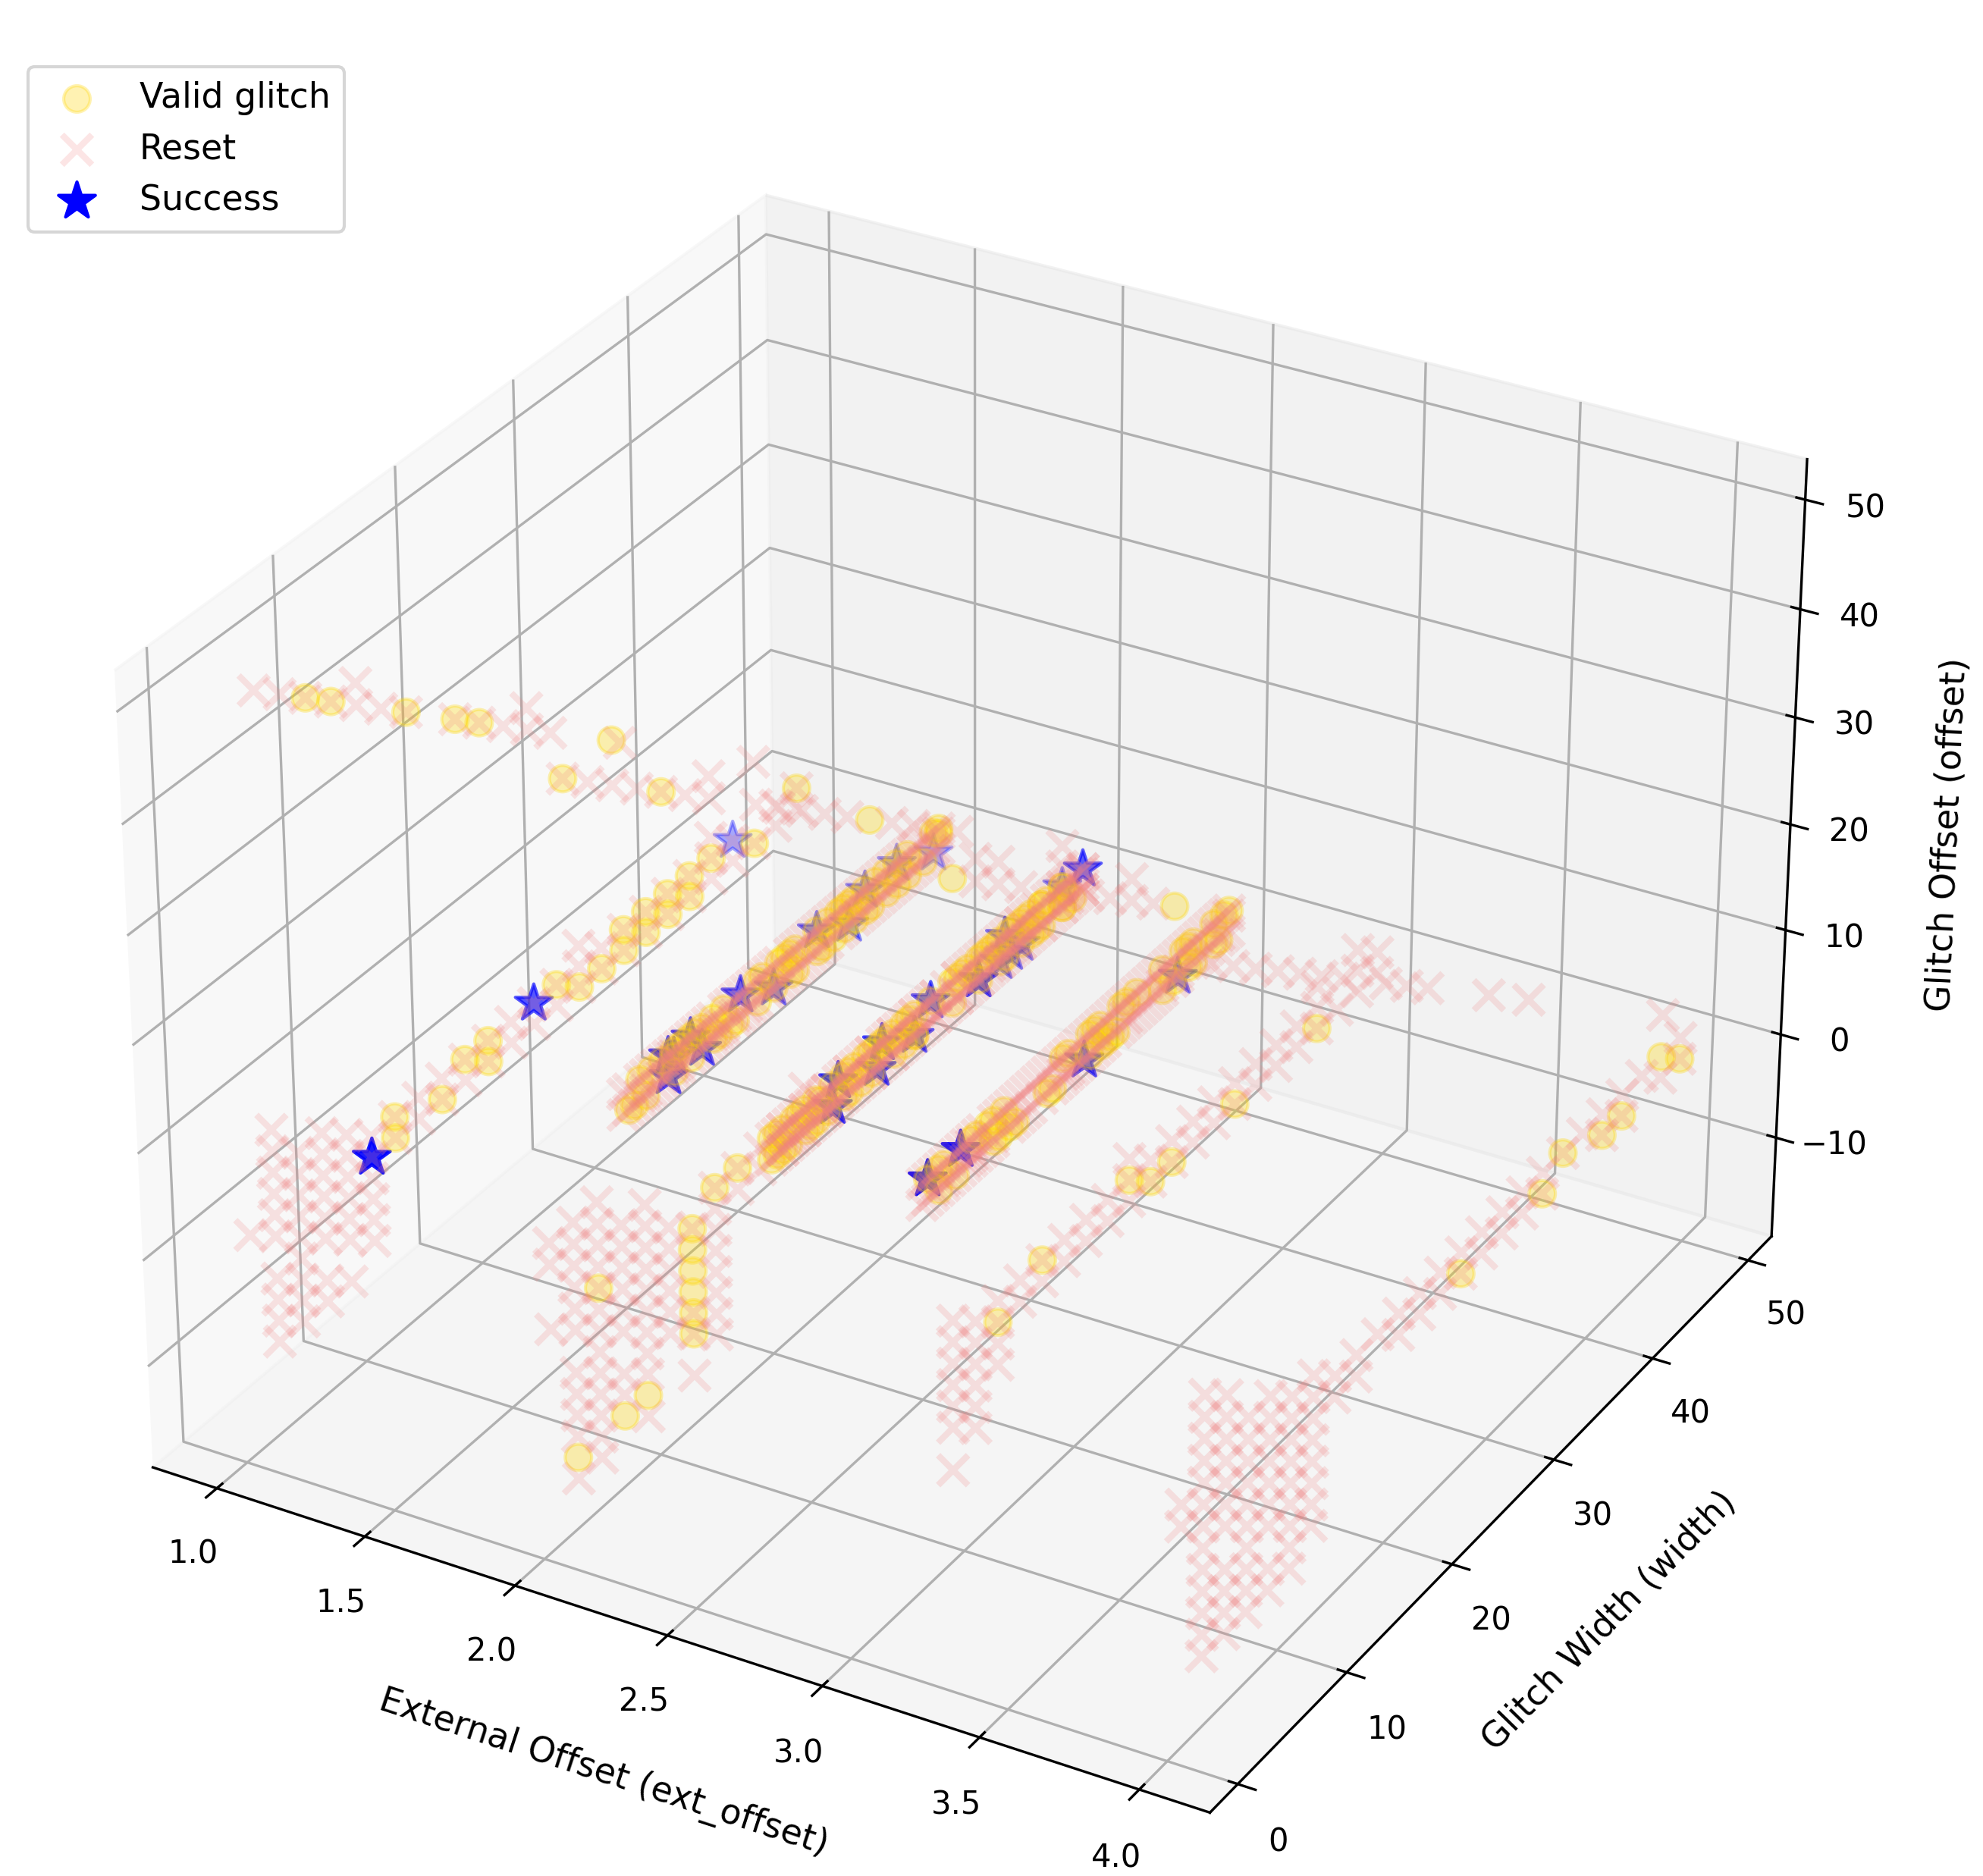
\includegraphics[width=0.56\textwidth]{content/images/glitch_3d_results_crop.png}
\caption{Model 1 (full tree disclosure): glitch outcome over
\texttt{ext\_offset}, \texttt{width} and \texttt{offset}, $10$ attempts per
parameter point. Blue stars mark successful faults, yellow circles
\emph{valid} glitches (runs that neither crashed nor produced the correct or
the target faulted path), pink crosses device resets.}
\label{fig:fault1_results}
\end{figure}

\textbf{Model 2: Subtree recovery.} We consider 
this attack successful if we obtain the faulted path pattern 
described by Figure~\ref{fig:faulted_path}. 

\textit{Compilation.} This is carried out on a code compiled with the default \texttt{-Os} optimization.

\textit{Trigger position.} The trigger frames \chg{line~\ref{lst:path:inc}} of
Listing~\ref{lst:path}; the compiled result is Listing~\ref{lst:f2asm} in
Appendix~\ref{app:asm}.

\textit{Parameters.} Evaluating the condition and incrementing \texttt{id}
take $3$ clock cycles, so we set \texttt{repeat} to $3$;
Figure~\ref{fig:fault2_results} gives the resulting success map. \chg{The best
point is \texttt{ext\_offset}$=2$, \texttt{offset}$=4$, \texttt{width}$=9$,
giving $23\%$ success over $100$ confirmatory attempts (Wilson $95\%$ CI
$[16\%,32\%]$) with a $62\%$ reset rate; these are the Model~2 row of
Table~\ref{tab:fault-success}.}

For Model~2 we observe a bounded region of system resets bordered by
successful attacks and other valid glitches, many of whose paths carry enough
intermediate nodes to recompute every leaf.

\textbf{Model 3: Single hidden leaf recovery.} Here only one hidden leaf is
disclosed.

\textit{Compilation.} At \texttt{-O1} and above, including \texttt{-Os}, the
compiler removes the explicit assignment and achieves the same outcome through
control flow, leaving nothing precise to target. We therefore build the target
function at \texttt{-O0}; applying \texttt{-O0} project-wide overflows the
board's flash.

\textit{Trigger position.} On the unoptimised build we place the high trigger
immediately before the \texttt{index\_leaf} assignment and the low trigger
immediately after; the compiled result is Listing~\ref{lst:f3asm} in
Appendix~\ref{app:asm}.

\textit{Parameters.} The disassembly shows the assignment compiled to two
single-cycle instructions, so we set \texttt{repeat} to $2$;
Figure~\ref{fig:fault3_results} gives the success map. \chg{The best point is
\texttt{ext\_offset}$=7$, \texttt{offset}$=3$, \texttt{width}$=8$, giving
$16\%$ success over $100$ confirmatory attempts (Wilson $95\%$ CI
$[10\%,24\%]$) with a $5\%$ reset rate; the hot band is confined to
\texttt{ext\_offset}$=7$.}

\begin{figure}[!tb]
\centering
\begin{subfigure}[b]{0.46\textwidth}
  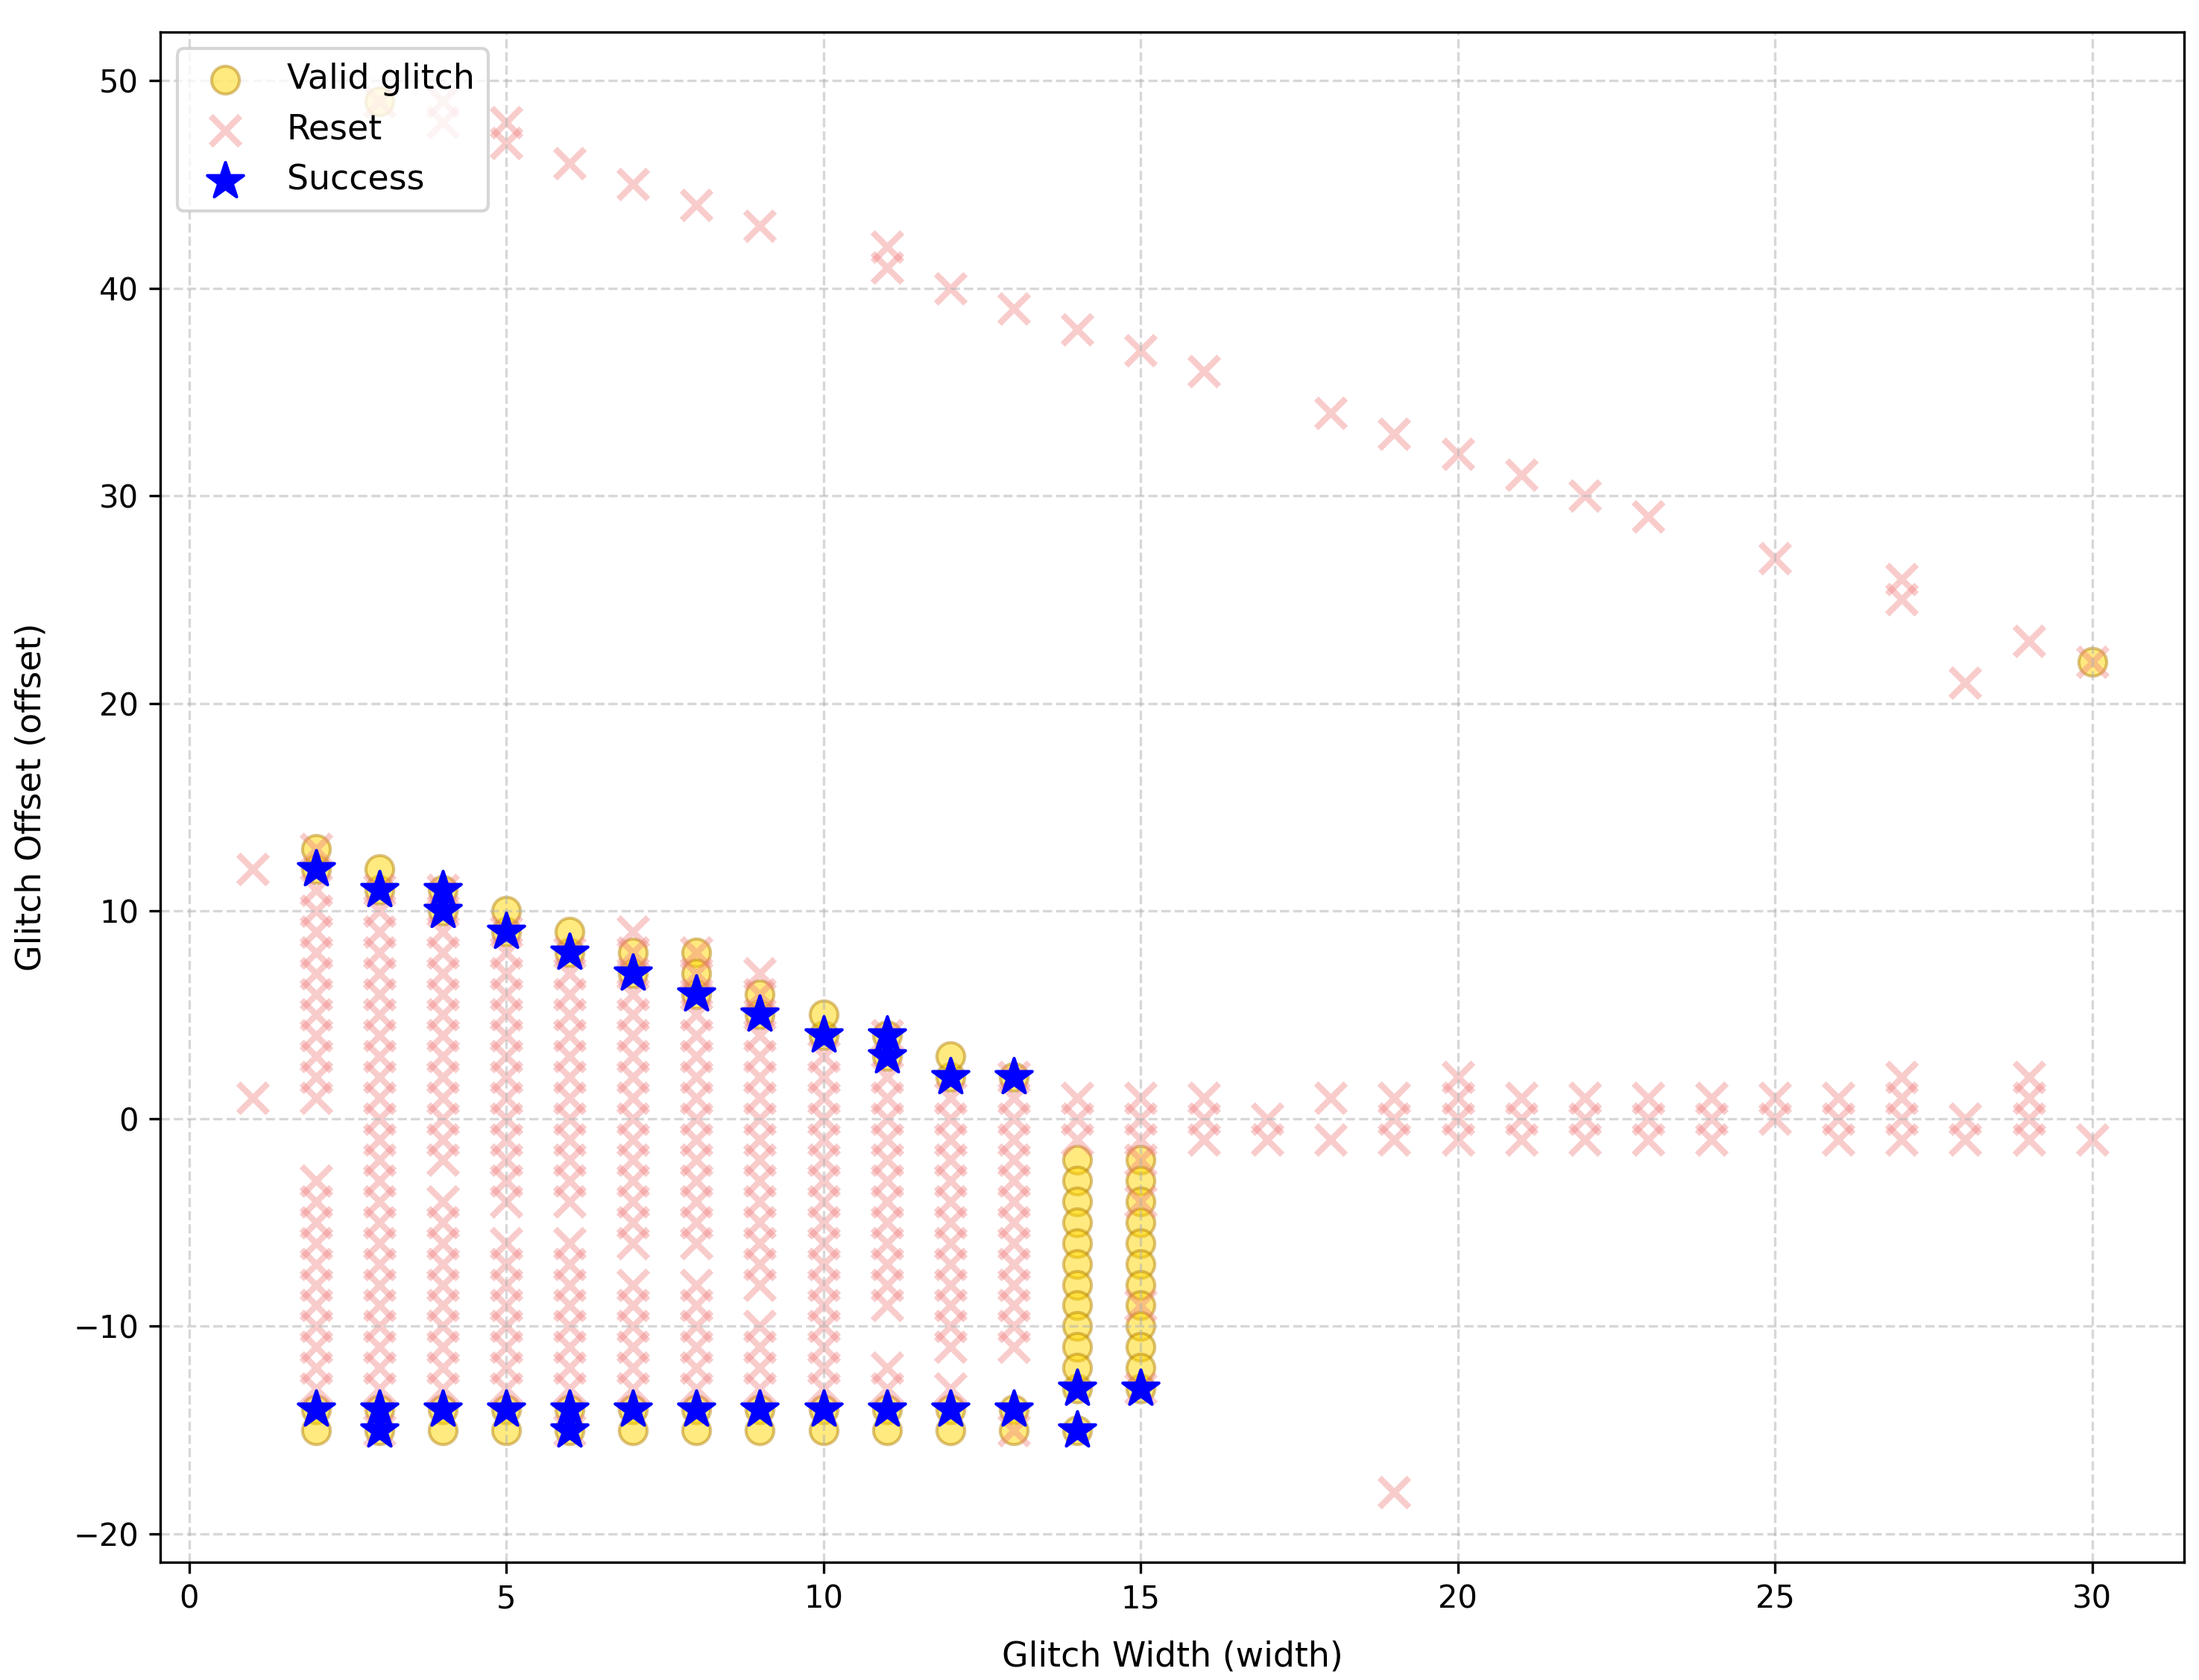
\includegraphics[width=\linewidth]{content/images/glitch_2d_results_ext2_crop.png}
  \caption{Model 2 (subtree), $\texttt{ext\_offset} = 2$.}
  \label{fig:fault2_results}
\end{subfigure}\hfill
\begin{subfigure}[b]{0.46\textwidth}
  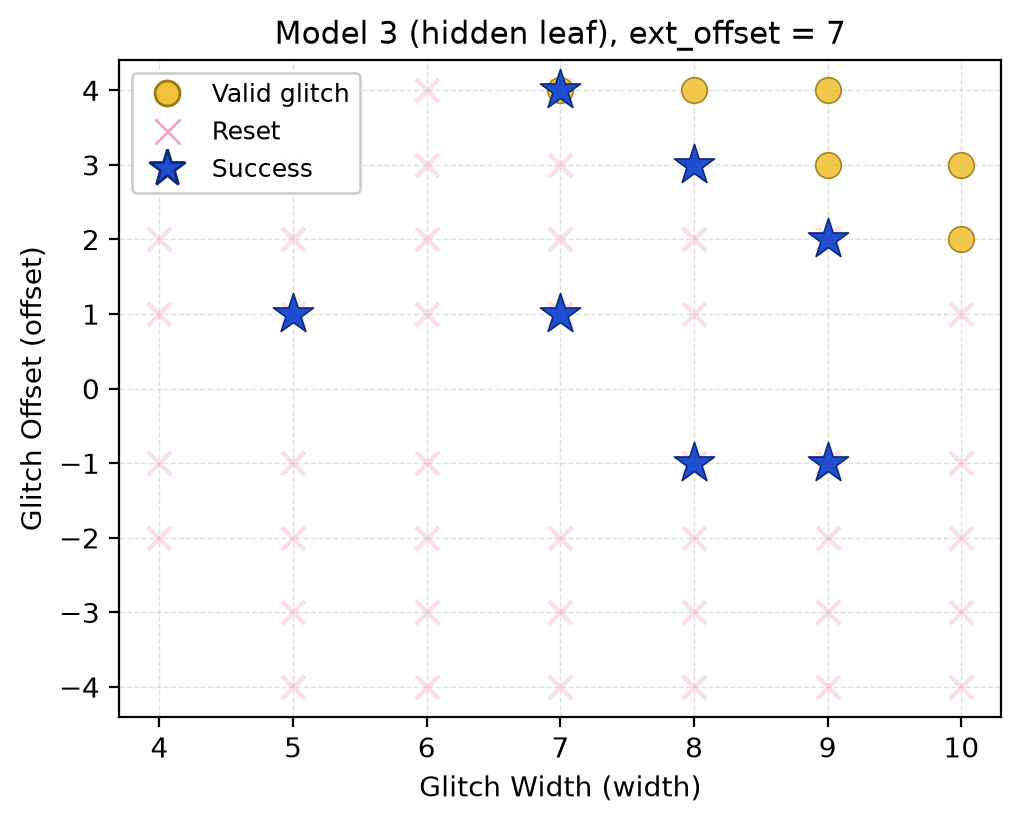
\includegraphics[width=\linewidth]{content/images/glitch_2d_results_ext7_crop.png}
  \caption{\chg{Model 3 (hidden leaf), $\texttt{ext\_offset} = 7$.}}
  \label{fig:fault3_results}
\end{subfigure}
\caption{Glitch success frequency for Models~2 and~3, $10$ attempts per
parameter point; markers as in Figure~\ref{fig:fault1_results}.}
\label{fig:glitch_results}
\end{figure}

\revon
\noindent\textbf{Results.} The target faulty outputs are reproducible under instrumentation. \chg{For Model~3, every
\revoff
attempt} gave normal execution, a device reset, or the expected exploit, with
no other valid glitches --- a consequence of single-instruction targeting,
which is less likely than a wider disruption window to bleed into surrounding
cycles\chg{; Models~1 and~2 also produce other valid glitches
(Figures~\ref{fig:fault1_results} and~\ref{fig:fault2_results})}. Model~1, the root reveal, is both the most efficient and the most
reproducible; Models~2 and~3 replicate less readily but are harder to detect
\revon
during signing (Section~\ref{sec:counter}).
\noindent\textbf{Limits of the evidence.}
The rates in Table~\ref{tab:fault-success} describe tuned points selected
after searching $672$, $1344$ and $448$ parameter combinations (ten trials
per point), not success probabilities for a previously unprofiled device.
Only Model~1 yields the full-tree disclosure required by the one-query
coverage calculation; Models~2--3 generally expose fewer hidden seeds.
Our tests did not reconstruct MEDS response pairs from a full emitted
signature, demonstrate key extraction on the target, or measure the ability
to hit the publication routine from the start of complete signing. Model~3
uses a non-default \texttt{-O0} build, so its transfer to the normal
\texttt{-Os} binary remains open.
\revoff
